\begin{figure}[H]
\centering
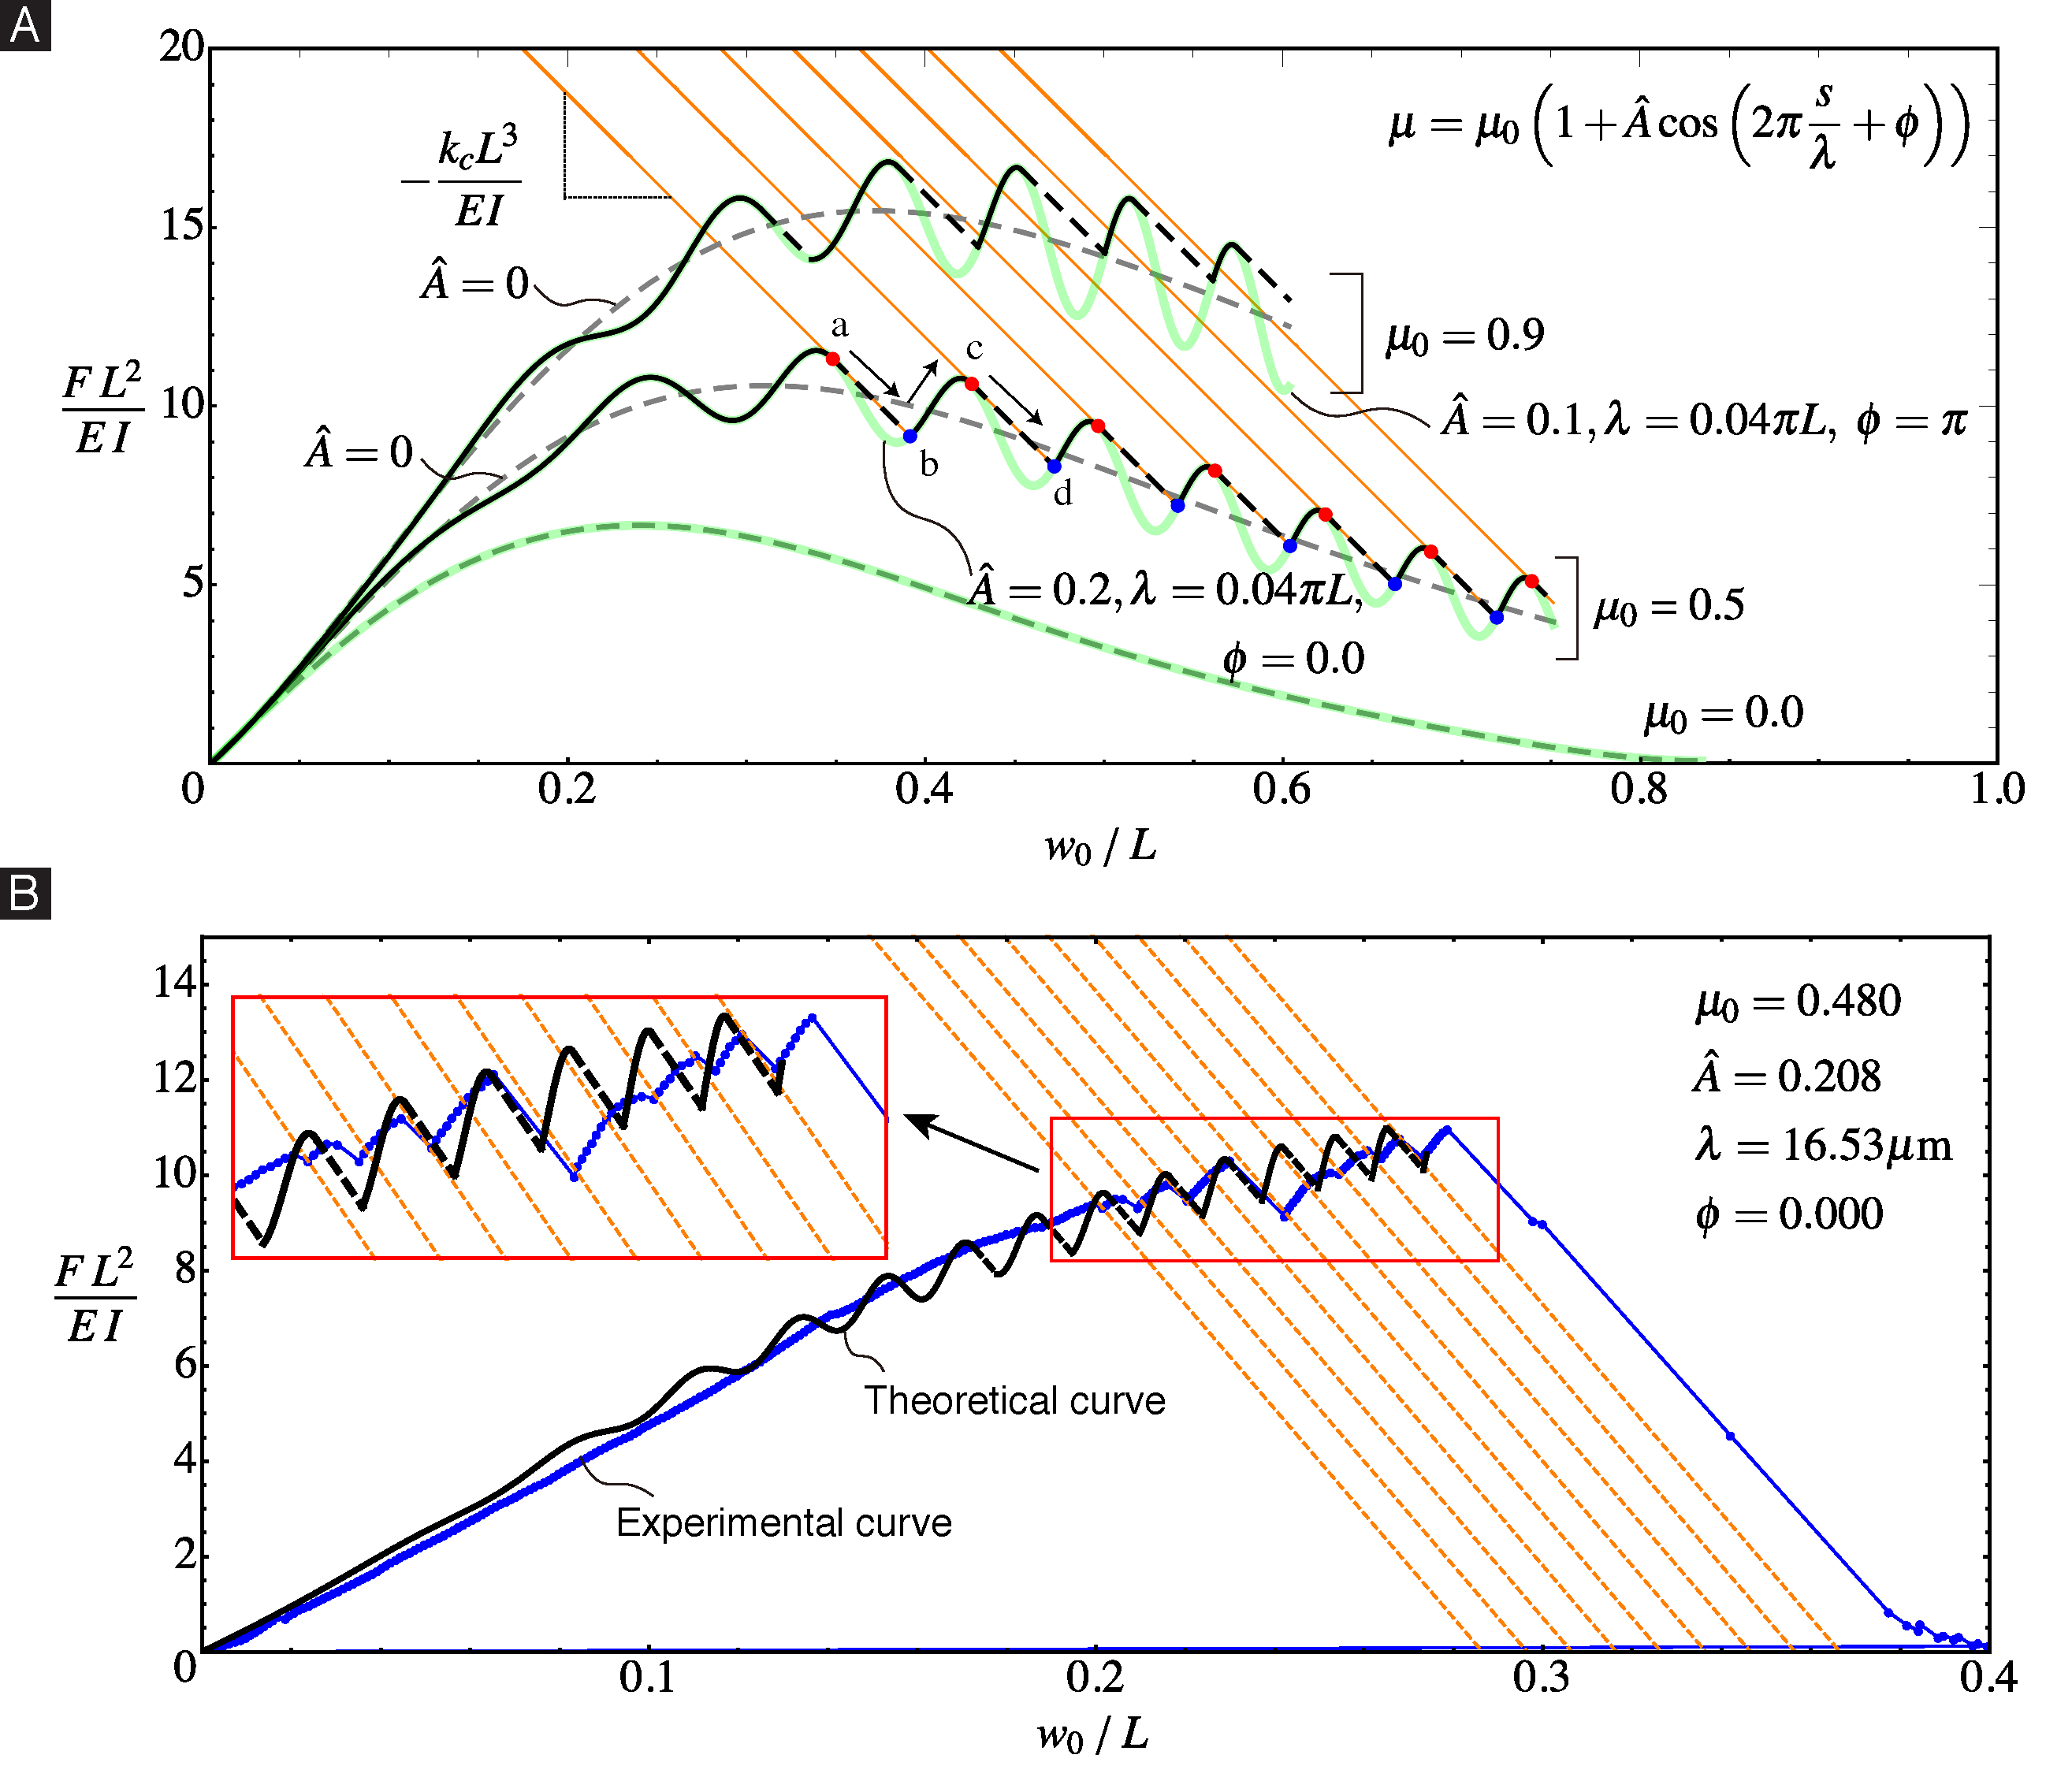
\includegraphics[width=0.9\textwidth]{Figures/Comparison.pdf}
\caption{
% Results of nonlinear bending-sliding model.
(\textsf{A}) A schematic of dimensionless force-deflection curves from nonlinear bending-sliding model. The equilibrium $\hat{F}$-$\hat{w}_0$ curves for constant $\mu = \mu_0$ are plotted as gray dashed lines, while the green lines are for sinusoidal $\mu$. The black lines denote the real $\hat{F}$-$\hat{w}_0$ response where the dashed parts are jumps. The orange oblique lines describe the $\hat{F}$-$\hat{w}_0$ relations of the cantilever, the loading device in the test, as stage displacement $w_s$ increases. The slope for these oblique lines is marked as $-\frac{k_c L^3}{E I}$. Red points and blues points denote the tangential points and intersections of the obliques lines and the green curves, respectively.
(\textsf{B}) A Representative comparison between the theoretical (black) and experimental (blue) $\hat{F}$-$\hat{w}_0$ response for test SS38. The orange oblique lines describe the $\hat{F}$-$\hat{w}_0$ relations of the cantilever, the loading device in the test, as stage displacement $w_s$ increases.
}
\label{fig:NBSComparison}
\end{figure}
